\documentclass[a4paper, 11pt]{article}

% --- Essential Packages ---
\usepackage[utf8]{inputenc}
\usepackage[english]{babel}
\usepackage{graphicx}
\usepackage{geometry}
\usepackage{setspace}
\usepackage{float}
\usepackage{caption}
\usepackage{titlesec}
\usepackage{mathptmx}
\usepackage{amsmath}
\usepackage{hyperref}
\usepackage{tikz}

% --- Page Setup ---
\geometry{a4paper, margin=2.5cm}
\setstretch{1.4}

% --- Section Styling ---
\titleformat{\section}{\large\bfseries}{\thesection}{1em}{}[\titlerule]
\titleformat{\subsection}{\normalsize\bfseries}{\thesubsection}{1em}{}

% --- Hyperlinks ---
\hypersetup{
	colorlinks=true,
	linkcolor=black,
	urlcolor=blue,
	citecolor=blue
}

\begin{document}
	
	% ==========================================
	% TITLE PAGE
	% ==========================================
	\begin{titlepage}
		\centering
		\vspace*{0.5cm}
		
\includegraphics[width=0.35\textwidth]{Resources/UNIPD_Logo}\\[1cm] 
		
		{\large \textsc{University of Padova}} \\
		{\small Department of Information Engineering} \\
		\vspace{1.5cm}
		
		{\Large \textbf{COMPUTER VISION - PROJECT 2}} \\
		\vspace{0.8cm}
		{\huge \textbf{Vision-Based ADAS Dashboard}} \\
		\vspace{0.4cm}
		{\large \textit{Classical Computer Vision vs. Hybrid Deep Learning}} \\
		
		\vspace{2.5cm}
		
		\begin{minipage}{0.45\textwidth}
			\begin{flushleft} \large
				\emph{Professor:}\\
				\textbf{Prof. Zanuttigh}
			\end{flushleft}
		\end{minipage}
		\hfill
		\begin{minipage}{0.45\textwidth}
			\begin{flushright} \large
				\emph{Student:}\\
				\textbf{Kiavash Rabbani Soudabi} \\
				ID: 2141822    
			\end{flushright}
		\end{minipage}
		
		\vfill
		{\large Academic Year 2025-2026}
	\end{titlepage}
	
	% ==========================================
	% TABLE OF CONTENTS
	% ==========================================
	\pagenumbering{roman}
	\tableofcontents
	\newpage
	
	\pagenumbering{arabic}
	\setcounter{page}{1}
	
	% ==========================================
	% SECTION 1: INTRODUCTION
	% ==========================================
	\section{Introduction \& Academic Context}
	
	\subsection{Abstract \& Project Objectives}
	Advanced Driver Assistance Systems (ADAS) are at the core of modern vehicle safety, and this project involved building a working vision-based pipeline that processes real dash-cam footage. The system was designed around four main tasks:
	\begin{itemize}
		\item \textbf{Lane Detection:} Extracting the drivable road boundaries.
		\item \textbf{Lane Classification:} Mathematically distinguishing between "solid" and "dashed".
		\item \textbf{Forward Collision Warning (FCW):} Detecting surrounding vehicles and estimating their proximity to trigger safety alerts.
		\item \textbf{Lane Departure Warning (LDW):} Monitoring the host vehicle's lateral drift and warning the driver before a potential lane crossing.
	\end{itemize}
	
	\textbf{Design Philosophy:} In real-world ADAS products, end-to-end deep learning models like LaneNet dominate lane extraction, since they handle noise and lighting variation far better than hand-tuned thresholds. That said, leaning entirely on a neural network black-box means skipping over the foundational principles. For that reason, I chose a \textbf{hybrid architecture}: YOLO handles object detection because that is genuinely where deep learning shines, while everything related to lane extraction -- color filtering, edge gradients, geometric clustering -- was built from classical computer vision primitives.
	
	\subsection{The Hybrid Pipeline Architecture}
	Each video frame passes through the following stages in order:
	\begin{enumerate}
		\item \textbf{Illumination Normalization:} Correcting harsh shadows using adaptive histogram equalization (CLAHE).
		\item \textbf{Feature Masking:} Fusing color thresholds with directional edge gradients.
		\item \textbf{Dynamic ROI \& Vehicle Blackout:} Cropping out background clutter and masking detected vehicles so their edges do not pollute the lane signal.
		\item \textbf{Geometric Extraction:} Running the Probabilistic Hough Transform to recover line segments.
		\item \textbf{DBSCAN Clustering:} Grouping raw segments into lanes and deciding whether each one is dashed or solid.
		\item \textbf{Temporal Memory:} Smoothing lane positions across frames with an Exponential Moving Average (EMA).
		\item \textbf{ADAS HUD:} Computing distances and lateral drift to drive the FCW and LDW visual overlays.
	\end{enumerate}
	
	\begin{figure}[h!]
		\centering
		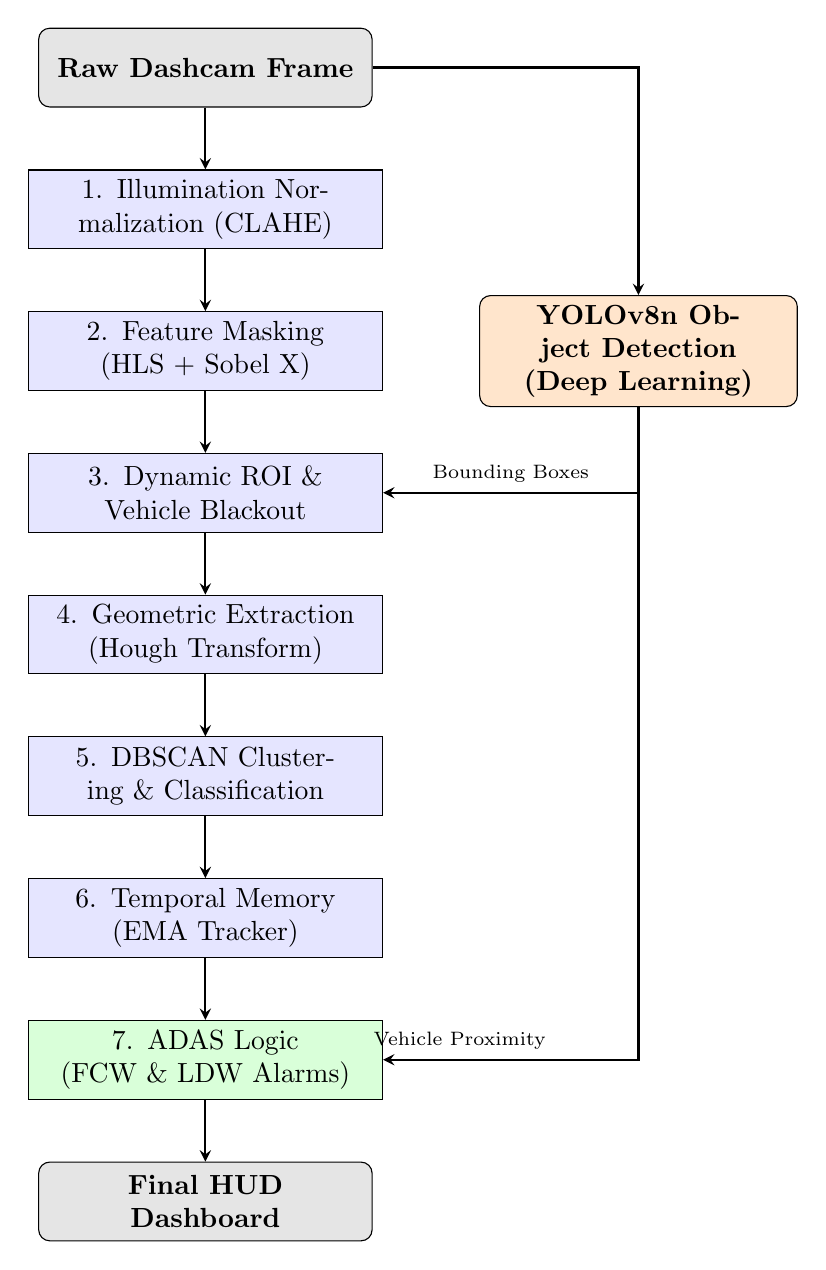
\begin{tikzpicture}[
			startstop/.style={rectangle, rounded corners, minimum width=4cm, minimum height=1cm, text centered, text width=4cm, draw=black, fill=gray!20, font=\bfseries},
			cvbox/.style={rectangle, minimum width=4.5cm, minimum height=1cm, text centered, text width=4.2cm, draw=black, fill=blue!10},
			aibox/.style={rectangle, rounded corners, minimum width=4cm, minimum height=1cm, text centered, text width=3.8cm, draw=black, fill=orange!20, font=\bfseries},
			hudbox/.style={rectangle, minimum width=4.5cm, minimum height=1cm, text centered, text width=4.2cm, draw=black, fill=green!15},
			arrow/.style={thick, ->, >=stealth} 
			]
			
			\node (input) at (0, 0) [startstop] {Raw Dashcam Frame};
			\node (clahe) at (0, -1.8) [cvbox] {1. Illumination Normalization (CLAHE)};
			\node (mask) at (0, -3.6) [cvbox] {2. Feature Masking \\ (HLS + Sobel X)};
			\node (yolo) at (5.5, -3.6) [aibox] {YOLOv8n Object Detection (Deep Learning)};
			\node (blackout) at (0, -5.4) [cvbox] {3. Dynamic ROI \& Vehicle Blackout};
			\node (hough) at (0, -7.2) [cvbox] {4. Geometric Extraction \\ (Hough Transform)};
			\node (dbscan) at (0, -9.0) [cvbox] {5. DBSCAN Clustering \& Classification};
			\node (ema) at (0, -10.8) [cvbox] {6. Temporal Memory \\ (EMA Tracker)};
			\node (adas) at (0, -12.6) [hudbox] {7. ADAS Logic \\ (FCW \& LDW Alarms)};
			\node (output) at (0, -14.4) [startstop] {Final HUD Dashboard};
			
			\draw [arrow] (input) -- (clahe);
			\draw [arrow] (clahe) -- (mask);
			\draw [arrow] (input.east) -| (yolo.north);
			\draw [arrow] (mask) -- (blackout);
			\draw [arrow] (yolo.south) |- (blackout.east) node[pos=0.75, above, text width=2cm, align=center, font=\scriptsize] {Bounding Boxes};
			\draw [arrow] (blackout) -- (hough);
			\draw [arrow] (hough) -- (dbscan);
			\draw [arrow] (dbscan) -- (ema);
			\draw [arrow] (ema) -- (adas);
			\draw [arrow] (yolo.south) |- (adas.east) node[pos=0.85, above, font=\scriptsize] {Vehicle Proximity};
			\draw [arrow] (adas) -- (output);
			
		\end{tikzpicture}
		\caption{Flowchart of the ADAS pipeline showing the classic CV and deep learning components.}
		\label{fig:pipeline}
	\end{figure}
	
	\subsection{Environment \& Tools}
	The pipeline was built in Python. The main libraries used are:
	\begin{itemize}
		\item \textbf{OpenCV \& NumPy:} The workhorses for matrix operations, filtering, and HUD rendering.
		\item \textbf{Scikit-Learn:} Brought in specifically for DBSCAN.
		\item \textbf{YOLOv8n:} The deep learning backend for detecting cars and trucks in real time.
	\end{itemize}
	
	% ==========================================
	% SECTION 2: PRE-PROCESSING
	% ==========================================
	\section{Overcoming Classical CV Limitations}
	One of the first things you realize when working with classical computer vision is how fragile it gets once the lighting changes. Deep learning models generalize across environments because they have seen thousands of varied training examples; classical pipelines do not have that luxury and depend heavily on absolute pixel values staying consistent. A shadow cutting across the road is enough to break a static threshold entirely. Most of the pre-processing phase was designed with exactly this problem in mind.
	
	\subsection{Illumination Normalization (CLAHE)}
	Standard RGB is a poor choice when illumination fluctuates, because luminance is entangled with the color channels. A yellow lane marker in direct sun and the same marker under a tree's shadow can produce pixel values so different that a single threshold fails to catch both.
	
	My approach was to convert each frame to the LAB color space, which separates luminance into its own channel (L), and then run CLAHE (Contrast Limited Adaptive Histogram Equalization) on that channel alone. The key advantage is that CLAHE boosts local contrast in a controlled way -- it brings out lane markings that are buried in dark regions without blowing out the brighter areas of the frame.
	
	\begin{figure}[h!]
		\centering
		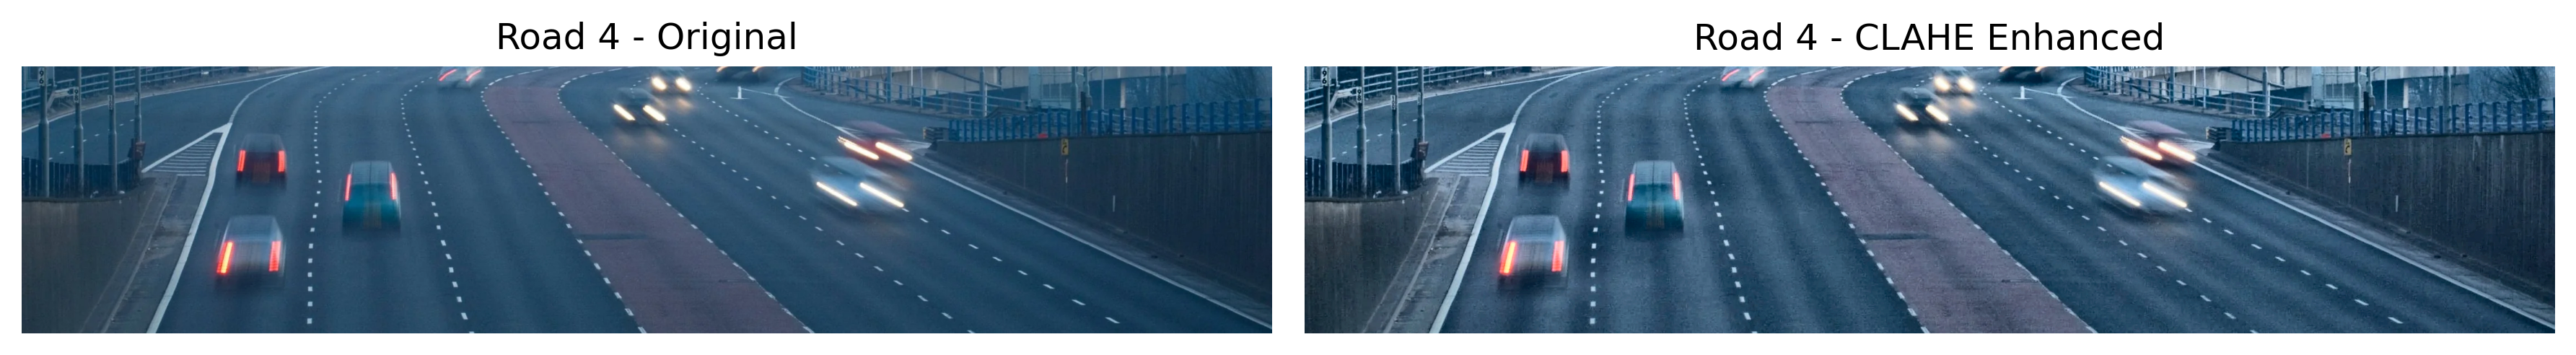
\includegraphics[width=1\textwidth]{Resources/clahe_comparison_road4.png}
		\caption{How CLAHE recovers road lines that are hidden in dark shadows.}
		\label{fig:clahe_comparison}
	\end{figure}
	
	\subsection{Directional Masking: Sobel Over Canny}
	My initial instinct was to use Canny edge detection, which is the default choice for most edge-based pipelines. After some testing though, it became clear that Canny picks up far too much: horizontal road cracks, crosswalk stripes, and the horizon line all show up with the same weight as lane markings, making it very noisy downstream.
	
	I switched to the Sobel X-gradient operator, which only computes the intensity derivative in the horizontal direction. This selectively highlights vertical edges -- exactly what lane lines look like from a forward-facing camera -- while horizontal structures are naturally suppressed. I then combined this Sobel mask with an HLS color threshold so that only edges matching the expected white or yellow paint colors would survive.
	
	\subsection{Parameterized ROI and "Vehicle Blackout"}
	White cars are a genuine problem for color-based lane detection. If a vehicle's side is bright and roughly vertical, the edge mask will pick it up, and the clustering step downstream will try to fit it as a lane.
	
	I dealt with this by adding a \textbf{Vehicle Blackout} step before any line extraction happens. Every frame is first run through YOLOv8n, and for each detected vehicle, the algorithm paints a black rectangle over the corresponding region on the edge mask. The lane extraction stage will bypass those pixels.
	
	On top of that, I applied a \textbf{Region of Interest (ROI)} crop. Rather than hard-coding pixel offsets, the ROI is defined as percentages of the frame's width and height, which makes it at least somewhat portable across different video resolutions.
	
	\textbf{A note on limitations:} The percentage-based ROI does help with resolution differences, but it is not truly adaptive. When I tested on frames captured with a camera mounted at a different angle, the ROI parameters needed manual adjustment. This kind of fragility is probably the most honest argument for why production systems rely on learned models rather than hand-crafted geometry.
	
	% ==========================================
	% SECTION 3: GEOMETRIC EXTRACTION
	% ==========================================
	\section{Geometric Lane Extraction}
	
	\subsection{Hough Transform \& Feature Space}
	With a clean binary edge mask in hand, the next step is finding actual line geometry. I used the Probabilistic Hough Transform (\texttt{cv2.HoughLinesP}) rather than the standard version, mainly because it is much faster -- it works by randomly sampling edge pixels rather than voting over the entire image.
	
	Tuning the parameters took some experimentation. Setting \texttt{minLineLength} high enough filters out the small reflective road markers, while \texttt{maxLineGap} controls whether broken dashed lines are bridged into a single segment or kept separate. Once the raw segments $(x_1, y_1, x_2, y_2)$ are extracted, each one is mapped to a compact 2D feature vector:
	
	\begin{itemize}
		\item \textbf{Angle (Slope):} Mainly used to throw out any remaining horizontal lines.
		\item \textbf{$X_{\text{bottom}}$ (Bottom Intercept):} The X-coordinate where the segment, when extended, crosses the bottom edge of the frame. Because of perspective projection, two parallel lanes will have nearly the same angle but clearly separated $X_{\text{bottom}}$ values, making this a reliable feature for distinguishing left from right.
	\end{itemize}
	
	\subsection{DBSCAN Clustering \& Paint Ratio}
	The Hough Transform typically returns dozens of short, overlapping fragments for a single physical lane marking. I grouped these using DBSCAN, which was a natural fit here for two reasons: the number of visible lanes is not constant (sometimes only one is clearly visible), and DBSCAN handles noise points gracefully by simply marking them as outliers rather than forcing them into a cluster.
	
	Before clustering, the features are normalized with \texttt{StandardScaler}. I also multiplied the $X_{\text{bottom}}$ feature by a factor of 7, deliberately biasing the algorithm so that physical position on the screen dominates the clustering decision over angle similarity. Without this weighting, segments from geometrically close but physically distinct lanes sometimes ended up in the same cluster.
	
	\textbf{Solid vs. Dashed Classification:} Rather than training a classifier, I used a simple geometric ratio. For each cluster, the algorithm sums the total painted segment length and divides it by the full vertical span of the lane on screen. I called this the ``Paint-Fill Ratio.'' A ratio above 85\% means the line is predominantly filled in, so it gets classified as ``Solid.'' Anything below that threshold is ``Dashed.''
	
	\begin{figure}[h!]
		\centering
		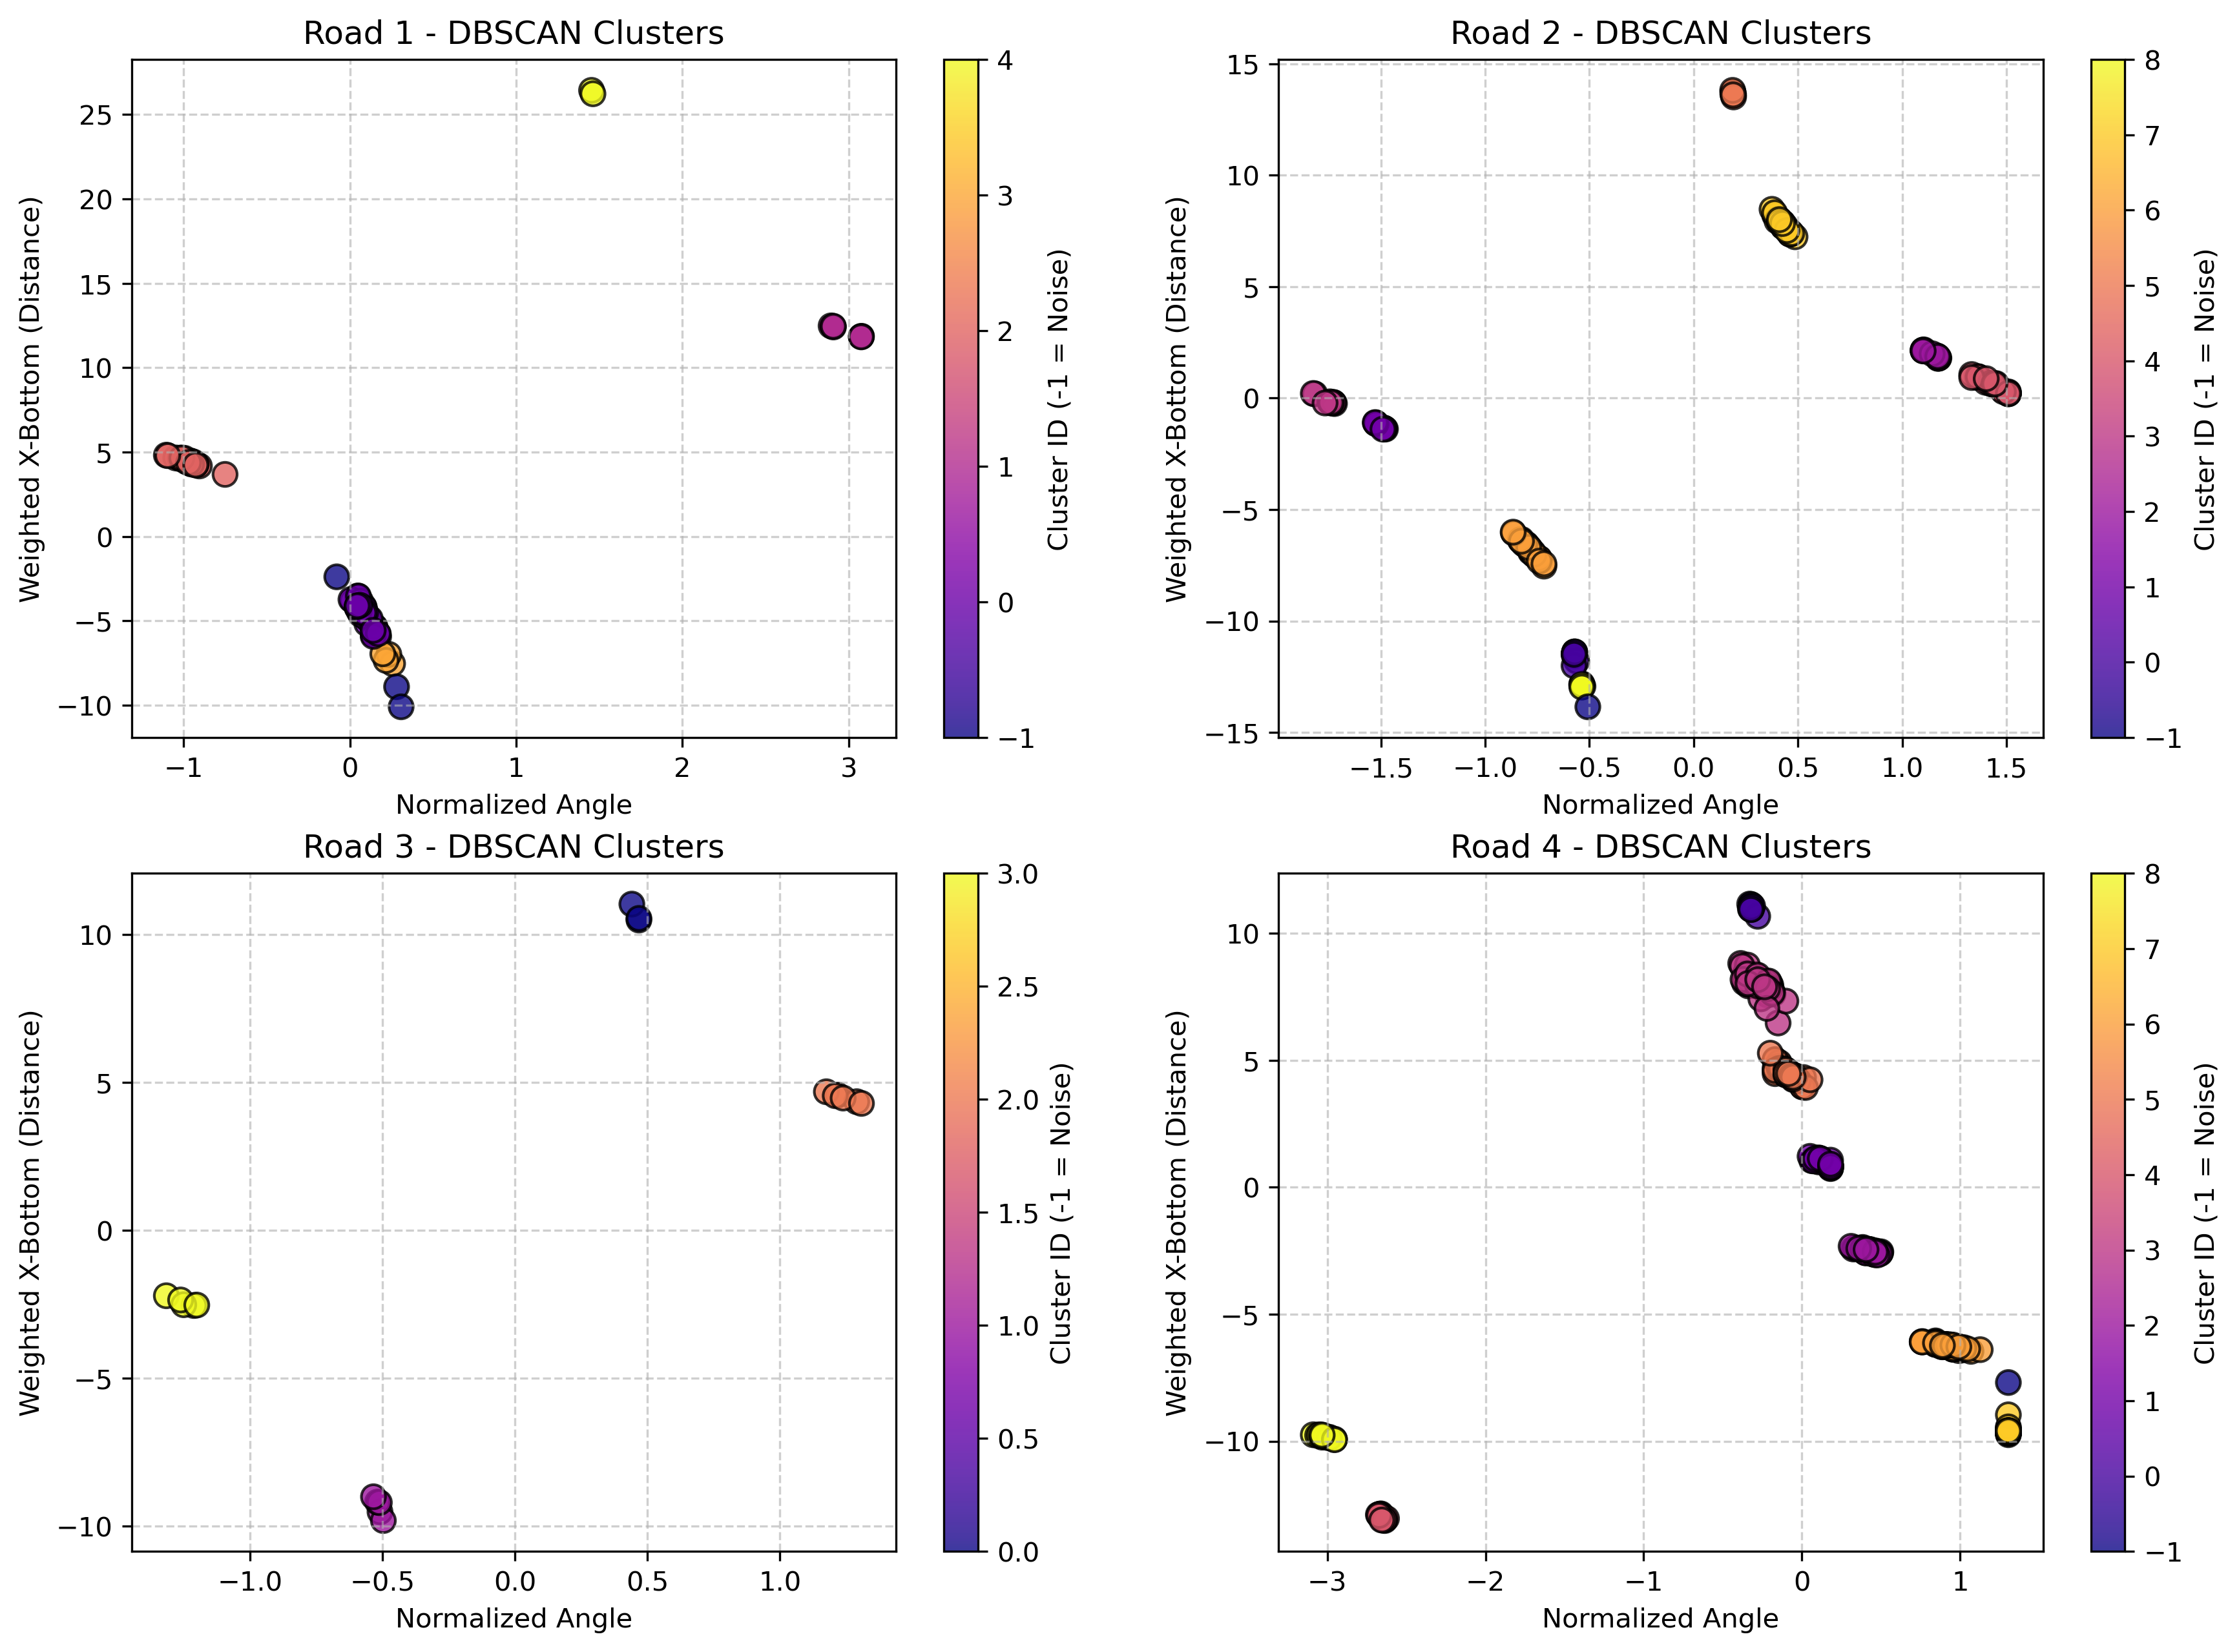
\includegraphics[width=0.8\textwidth]{Resources/scatter_plot.png}
		\caption{DBSCAN grouping the line segments based heavily on their $X_{\text{bottom}}$ position.}
		\label{fig:dbscan_scatter}
	\end{figure}
	
	\subsection{Resolving Flickering with Temporal Memory}
	Processing frames individually creates an annoying flickering effect: lanes disappear for a frame or two whenever lighting changes or a vehicle briefly occludes them, then reappear the next frame. Two mechanisms address this:
	
\begin{itemize}
	\item \textbf{Spatial Conflict Resolution:} When DBSCAN picks up both a lane marking and a concrete barrier on the same side, the system needs a way to decide which one to keep. The first check is slope: because of camera perspective, genuine lane lines appear steeper in the image than flat roadside structures, so the steeper candidate wins. If the two slopes are close enough that this test is inconclusive, the system falls back to proximity -- it keeps whichever cluster sits closer to the vehicle's center axis.
	
	\item \textbf{Temporal Tracker (EMA):} Lane positions are tracked across frames using an Exponential Moving Average. Rather than snapping to each new detection immediately, the stored position is nudged gradually:
	\[
	EMA_{\text{new}} = \alpha \cdot \text{Current}_{\text{pos}} + (1-\alpha) \cdot EMA_{\text{old}}
	\]
	When a lane goes undetected -- a passing truck briefly blocking the view is the typical case -- the tracker holds the last known position and keeps rendering it for up to 5 consecutive missing frames before dropping it. This single mechanism is responsible for most of the perceived smoothness in the final output.
\end{itemize}	
	
	% ==========================================
	% SECTION 4: ADAS FEATURES
	% ==========================================
	\section{Developing the ADAS HUD}
	Once reliable lane boundaries are in place, the remaining task is using that geometry to drive the safety alerts on the Heads-Up Display.
	
	\subsection{Drivable Area \& Asphalt Validation}
	The most visually prominent element on the HUD is a semi-transparent polygon filling the drivable corridor. The challenge is making sure this polygon is only drawn when the system is actually tracking valid lane geometry.
	
	I added a quick sanity check. Before drawing the overlay, the algorithm samples the average pixel color inside the bounded polygon and measures its distance from a dynamic reference color (calculated as the median color of all potential drivable areas in that specific frame). If the sampled color deviates too far from this dynamic baseline, the green fill is skipped entirely. It is a lightweight check, but it catches the most dangerous category of false positives while naturally adapting to changing lighting conditions.
	
	\subsection{Forward Collision Warning (FCW)}
	Without depth sensors, we need to find another way to calculate the distance of the other cars from the host. In a standard 2D perspective projection, objects that are farther away appear higher in the frame; closer objects have their bottom edge lower. This means the $Y_{\text{bottom}}$ coordinate of a vehicle's bounding box is a rough proxy for how close it is.
	
	The system tracks the $Y_{\text{bottom}}$ of any YOLO-detected vehicle whose bounding box intersects the drivable corridor. Once this value drops below a preset threshold -- meaning the car is close enough to be dangerous -- the bounding box turns red and a ``CAR TOO CLOSE'' banner is triggered on the HUD.
	
	\subsection{Lane Departure Warning (LDW)}
	The LDW logic relies on the $X_{\text{bottom}}$ coordinates that come out of the clustering stage. The vehicle's lateral position is estimated as the horizontal center of the frame ($Width / 2$), and the system continuously measures how far this center sits from the $X_{\text{bottom}}$ of each tracked lane. When the gap between the vehicle center and either lane boundary shrinks below a minimum margin (150 pixels in the current configuration), the system triggers a flashing ``LEFT LANE DRIFT'' or ``RIGHT LANE DRIFT'' alert.
	
	% ==========================================
	% FIGURES: FCW AND LDW
	% ==========================================
	\begin{figure}[h!]
		\centering
		\begin{minipage}{0.48\textwidth}
			\centering
			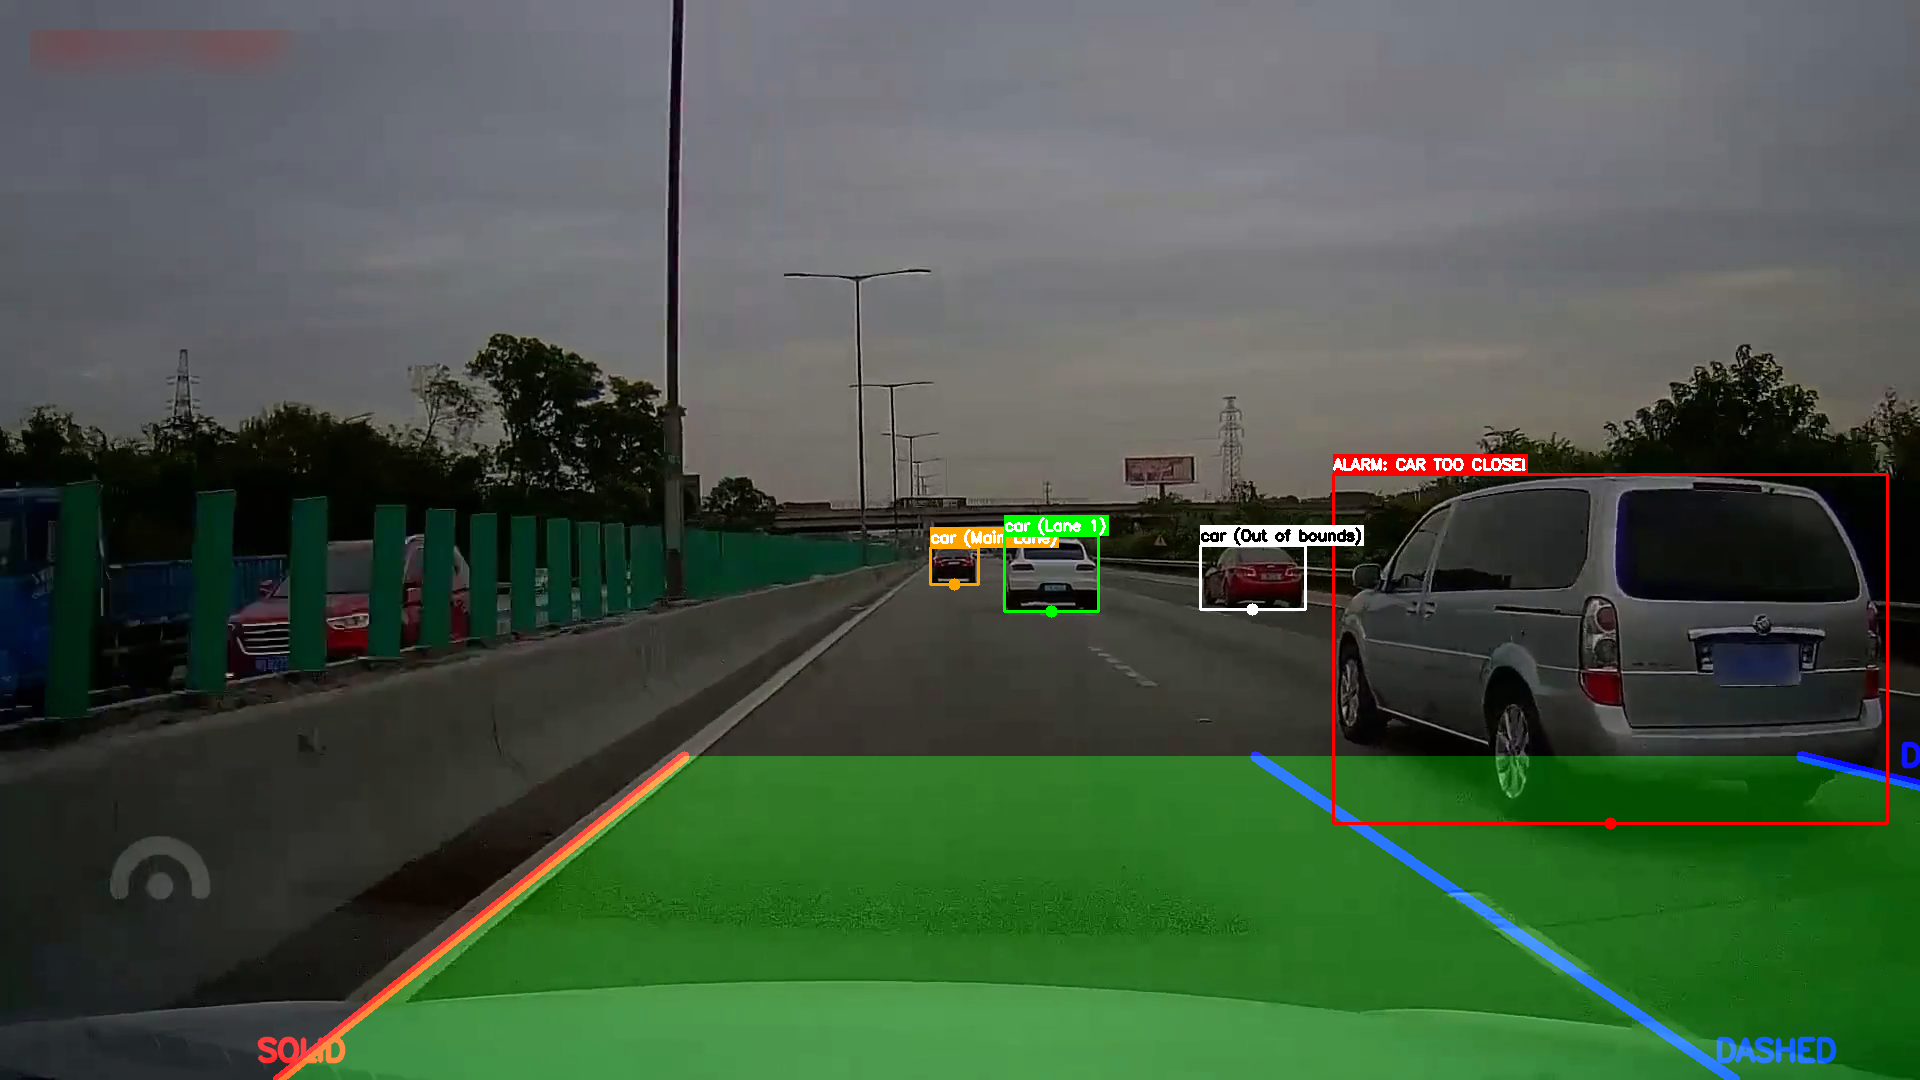
\includegraphics[width=\linewidth]{Resources/ForwardCollisionWarning.png}
			\caption{FCW alarm triggered when a detected vehicle becomes too close in the Y-axis.}
			\label{fig:fcw_warning}
		\end{minipage}\hfill
		\begin{minipage}{0.48\textwidth}
			\centering
			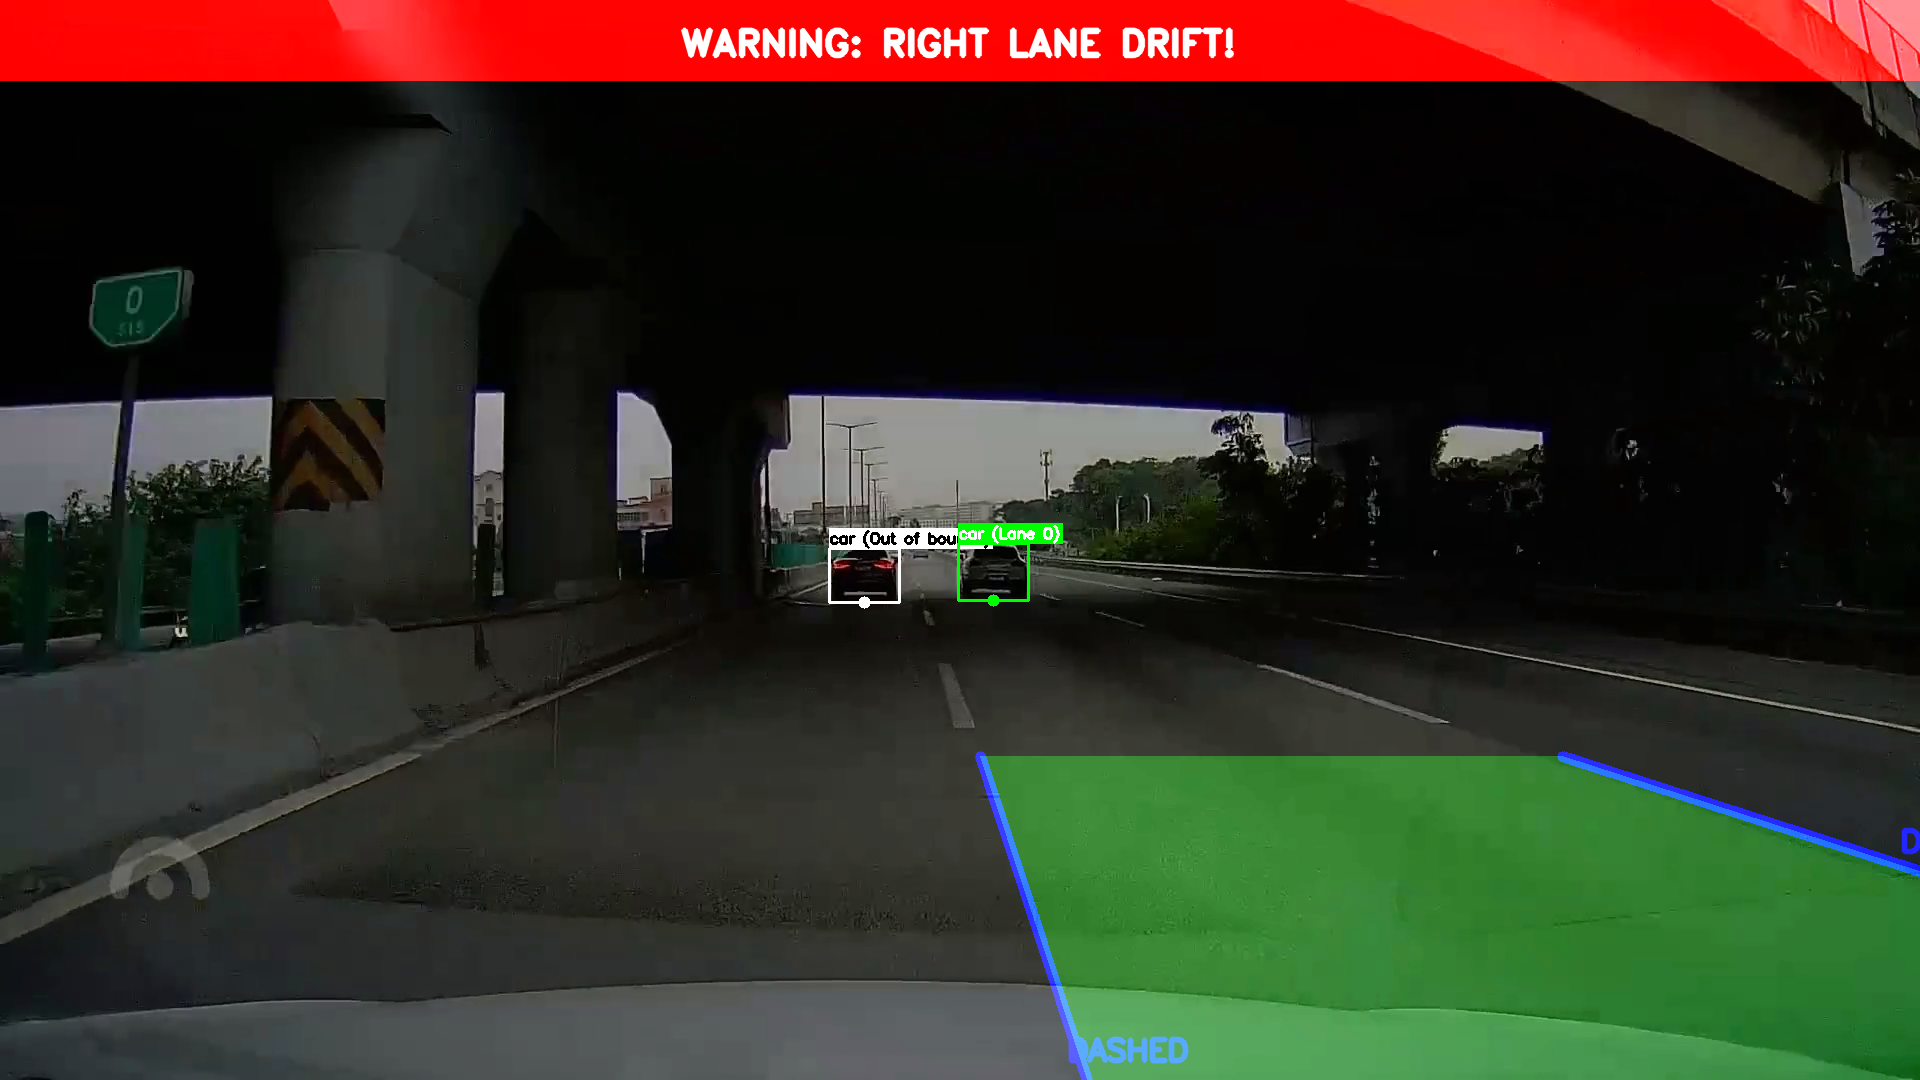
\includegraphics[width=\linewidth]{Resources/LaneDepartureWarning.png}
			\caption{LDW alarm triggered by lateral drift towards the right lane boundary.}
			\label{fig:ldw_warning}
		\end{minipage}
	\end{figure}
	
	% ==========================================
	% SECTION 5: CONCLUSION
	% ==========================================
	\section{System Evaluation and Conclusion}
	Under reasonable road conditions, the pipeline works well -- I estimate roughly 75\% reliability, meaning the lane overlay and ADAS alerts behave correctly on the majority of frames. Testing on messier footage exposed two clear weak points worth discussing.
	
	The first is speed. Running YOLOv8n inference and a full classical pipeline (CLAHE, Hough, DBSCAN) back to back in Python creates a real bottleneck. Any serious deployment would need either multithreading or a move to a lower-overhead language. The second limitation is curvature: because the lane model is linear ($y = mx + b$), the system starts to struggle on sharp bends where a polynomial fit would obviously be more appropriate.
	
	Looking back, the project was genuinely useful in making clear why industry has converged on semantic segmentation for this problem. A trained model does not need manual ROI tuning, does not break on shadows, and naturally handles curves -- all the things this pipeline had to work around explicitly. At the same time, going through the exercise of building the feature extraction, clustering, and temporal tracking logic from scratch gave a much more concrete understanding of what those learned representations are actually replacing.
	
	\begin{figure}[h!]
		\centering
		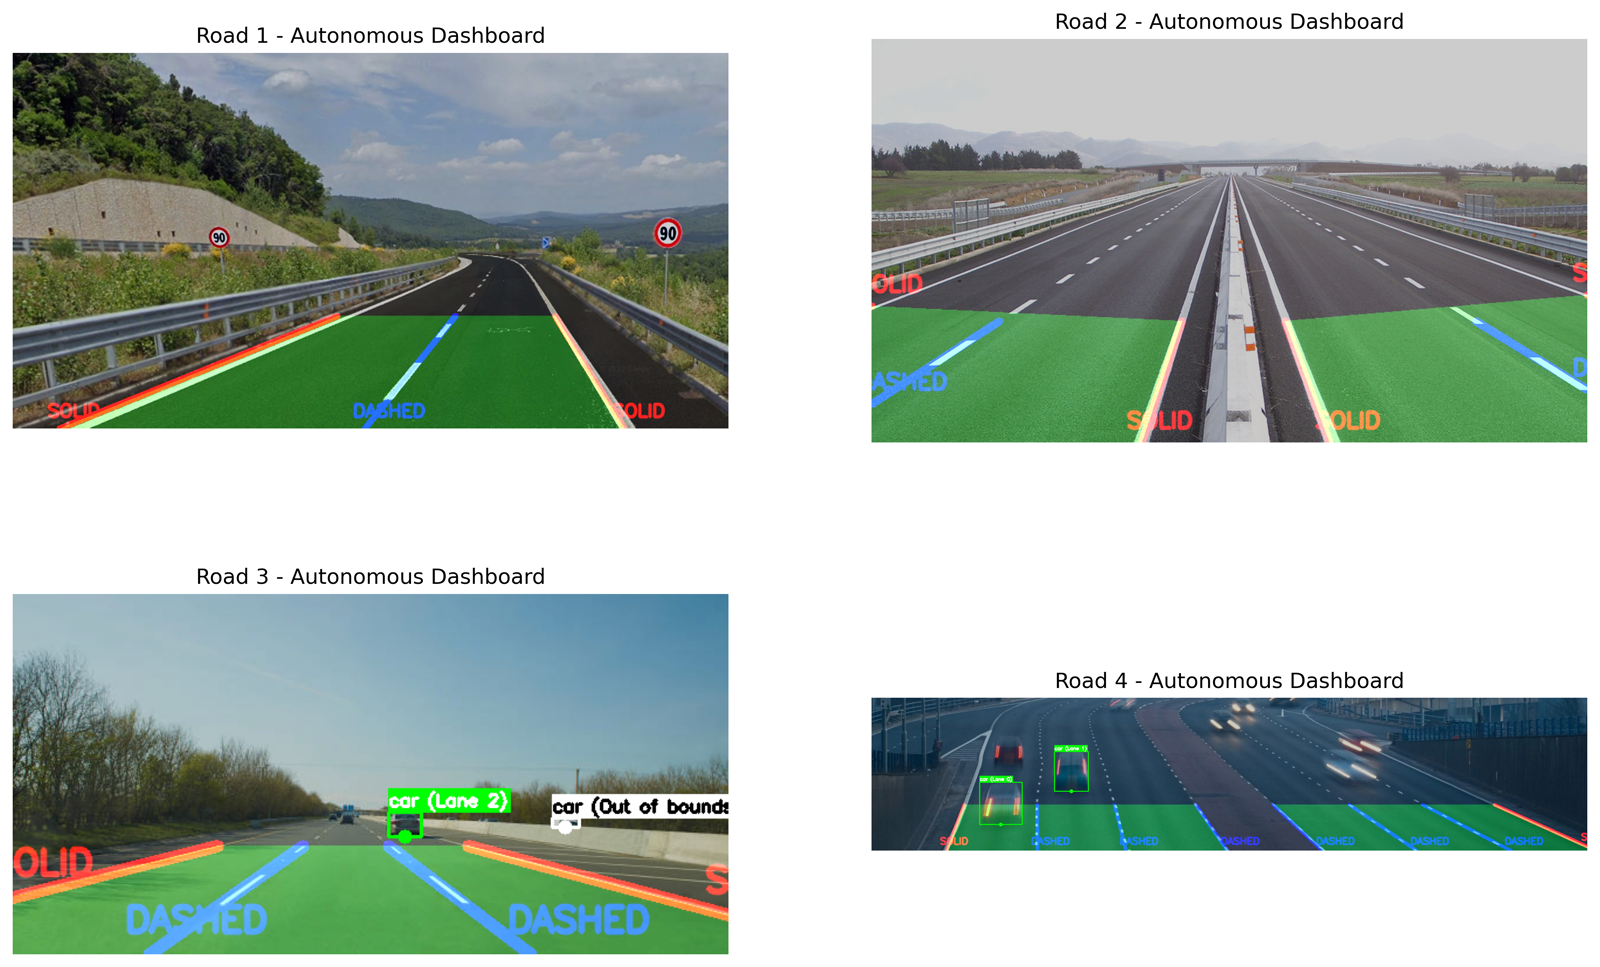
\includegraphics[width=0.9\textwidth]{Resources/finalResults.png}
		\caption{Evaluating the pipeline on test images, showing successful detection without relying on the temporal tracker.}
		\label{fig:final_results_static}
	\end{figure}
	
\end{document}